
\chapter{Software}
\label{Software}
\section{Arduino IDE on PC}
\label{Arduino Integrated Development Environment (IDE)}
\subsection{Installation}


Arduino Nano 33 BLE Sense uses the Arduino software integrated development environment (IDE) for programming, which is the most widely used and common (IDE) for all arduino boards that can be run online and offline. This is a open-source Arduino Software (IDE) simplifies code writing and upload to the board. Code created in the Arduino Software (IDE) is referred to as sketches. These sketches are composed in the text editor and saved using the .ino file extension.\cite{Arduino:2024e}. There are various version of software which can be installed in different operating system (OS) such as mac, linux, and windows.\cite{Arduino:2024f}. The Arduino community also provides coding online and save the sketches created in the cloud, this online Arduino IDE includes all libraries and also supports new Arduino boards. For getting access to these software packages go to the following link \url{https://www.arduino.cc/en/software}  and get more up to date information, as there are frequent updates. These software can be used with any Arduino board, the most recent offline arduino IDE 2.3.3 can be seen in Figure, \ref{fig:arduino-creat-agent-installieren} it is also supportive for all operating systems.\cite{Arduino:2024f}.

\begin{figure}[h]
	\centering
	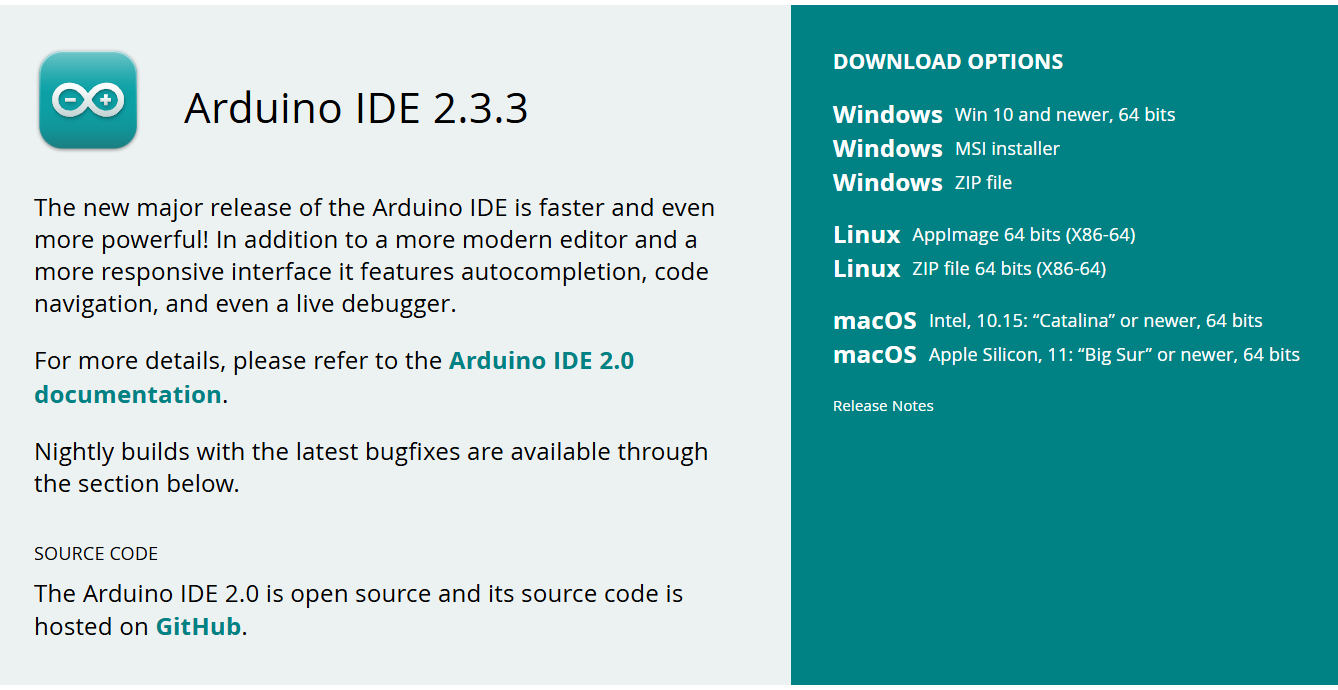
\includegraphics[width=0.7\textwidth]{Images/IDE_instal}
	\caption{Arduino IDE Installation}
	\label{fig:arduino-creat-agent-installieren}
\end{figure}


\subsection{Configuration}

To program the Arduino Nano 33 BLE Sense offline, the latest Arduino IDE needs to e installed in the desktop computer. After installation, to access the Arduino Nano 33 BLE Sense board, the IDE needs to be configured. The configuration can be completed by opening the IDE, navigate to tools which can be seen on the upper left corner in IDE screen; then select Board followed by Boards Manager. \cite{Arduino:2024g}. This selection will open a new window, with several available cores. Identify the one named Arduino Mbed OS Nano Boards and install it as shown in \ref {fig:Arduino-Mbed-Boards Installation}. The Mbed OS nano board supports also other nano family boards including Arduino nano 33 ble sense, after installing simply connect the Arduino Nano 33 BLE Sense to the computer via USB cable. \cite{Arduino:2024g}.

\begin{figure}[h]
	\centering
	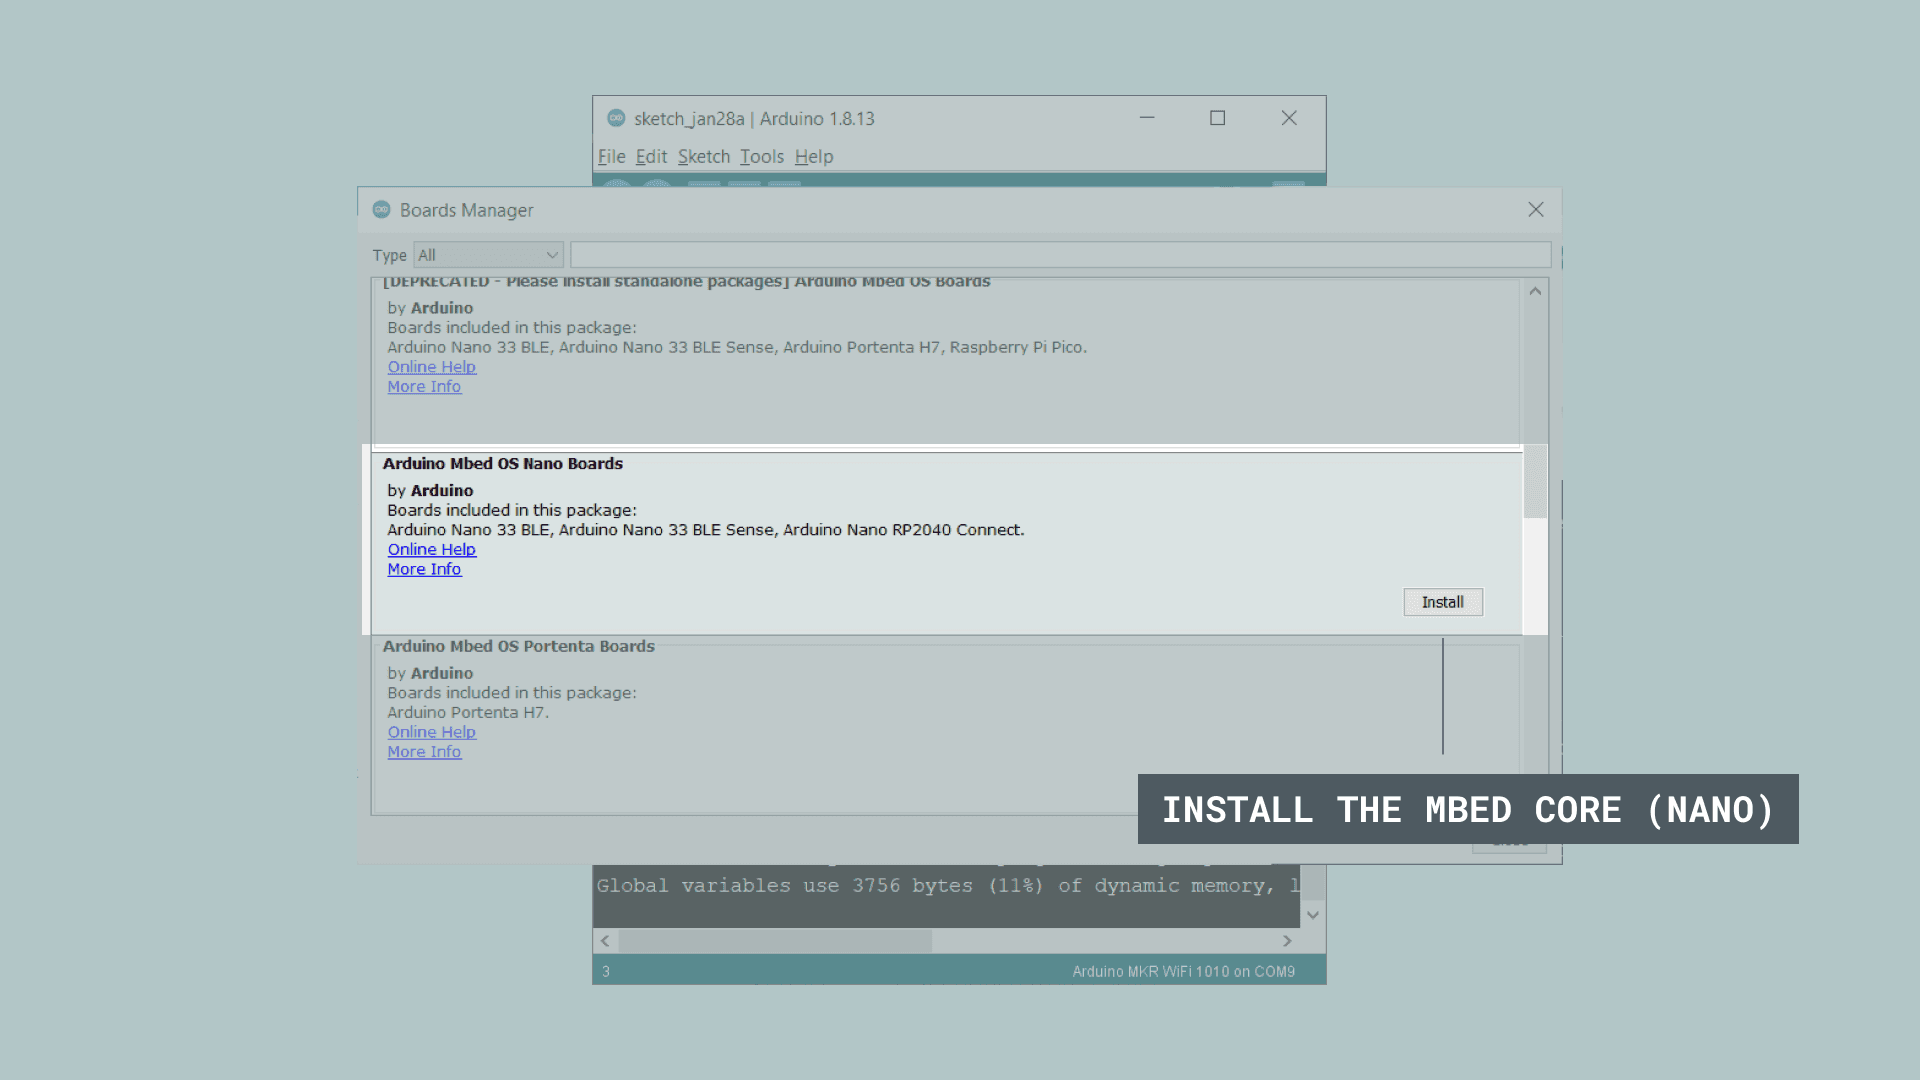
\includegraphics[width=0.7\textwidth]{Images/install_mbed_img03}
	\caption{Arduino Mbed OS Nano Boards Installation}
	\label{fig:Arduino-Mbed-Boards Installation}
\end{figure}


\subsection{Test Example}

There are set of examples which are available in Arduino (IDE) for the testing purposes. In order to check all the configurations and setting up the board we can open use the basic LED blink example as shown in the figure \ref{fig:LED-Example} \cite{Arduino:2024g}.

\begin{figure}[h]
	\centering
	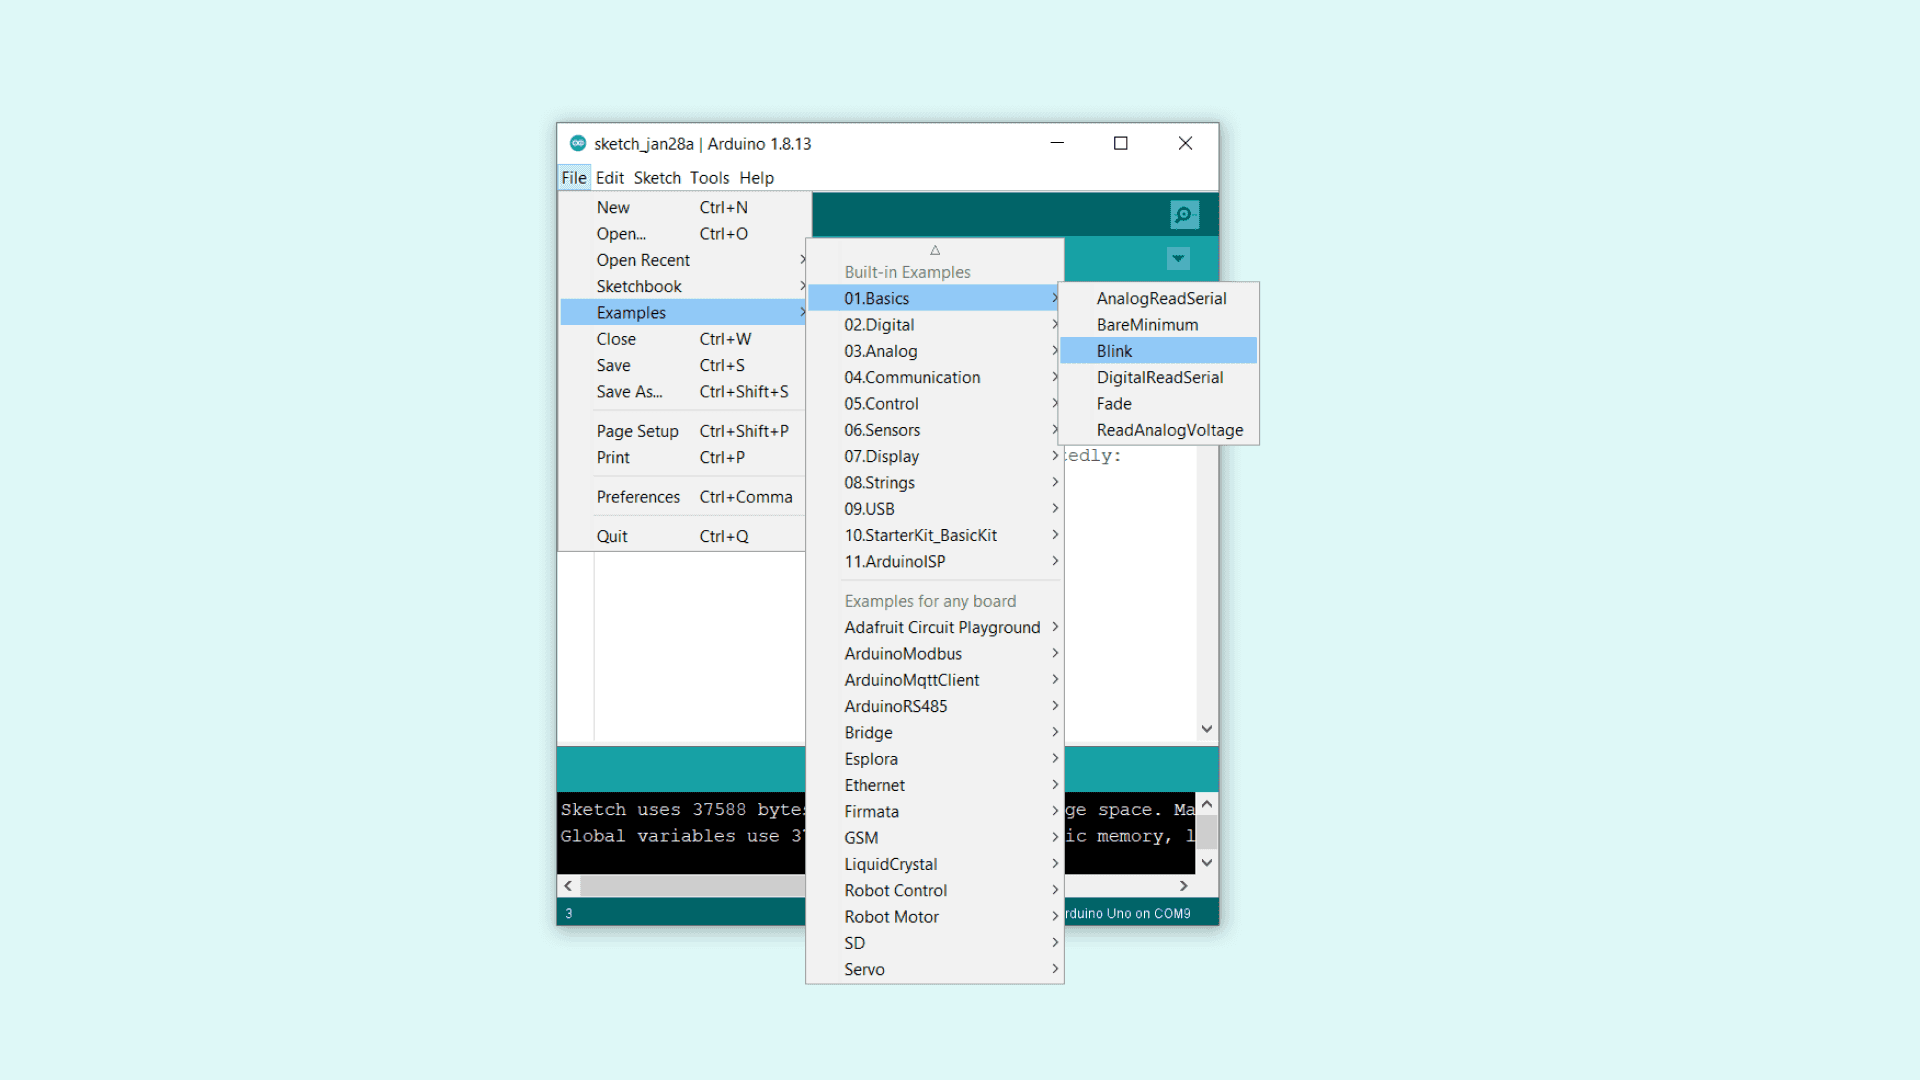
\includegraphics[width=0.7\textwidth]{Images/install_mbed_img06}
	\caption{Selecting the LED-Example Test}
	\label{fig:LED-Example}
\end{figure}
To upload the sketch, click on the arrow as shown in \ref{fig:LED-Example2}. It is critical that the board stays connected during the process. Once the code is uploaded, the wording "Done uploading." is displayed. At this point, an orange LED will blink on the board with an interval of one second. This signifies that the program was uploaded successfully to the board. \cite{Arduino:2024g}.
\begin{figure}[h]
	\centering
	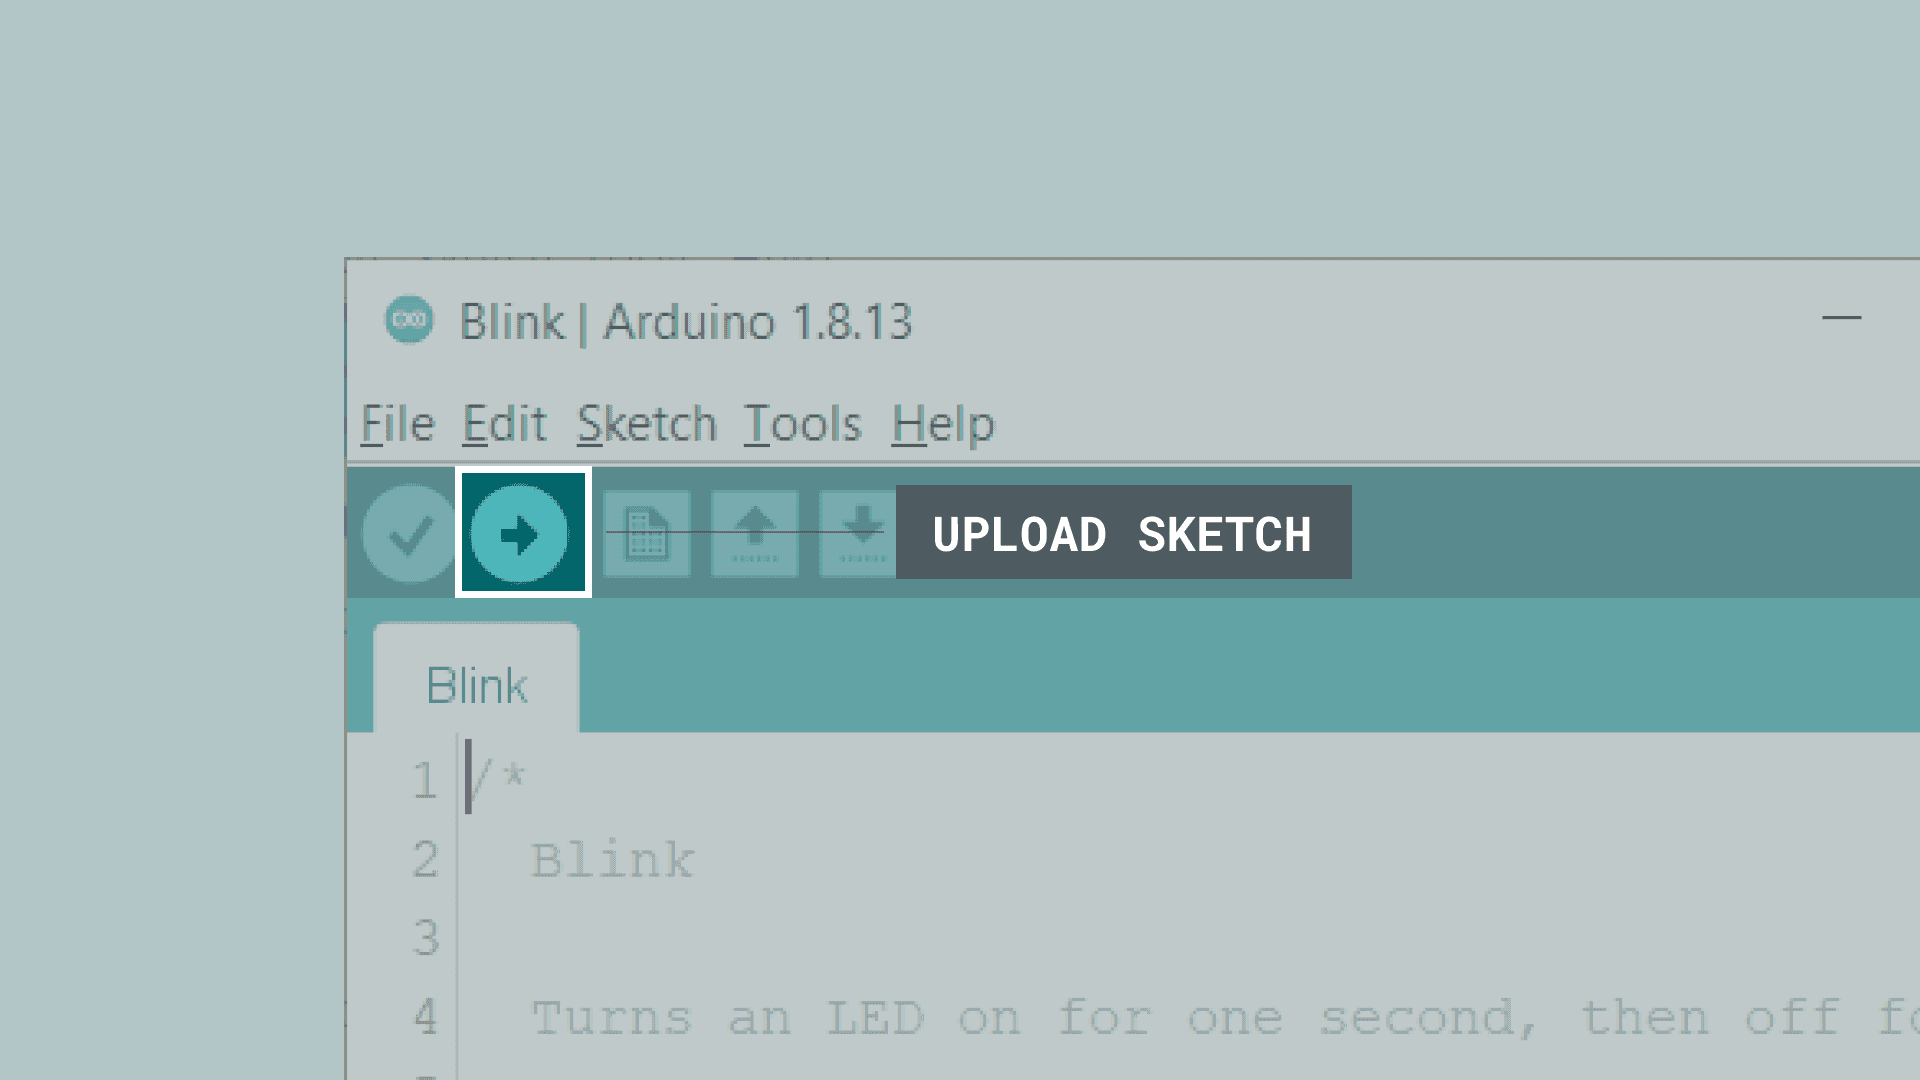
\includegraphics[width=0.7\textwidth]{Images/install_mbed_img07}
	\caption{Selecting the LED-Example Test}
	\label{fig:LED-Example2}
\end{figure}


\subsection{Pre -requisites for Uploading the program}
\label{Uploading the program} 
There are some steps needed to run the build in example or run one's own written program. In order to program an Arduino board with a Laptop with the help of USB connection, open the Arduino IDE on desktop, a blank arduino environment page with just a Void setup and void loop written on it will appear. This completed by navigating to Tools and selecting the board from the list as shown in the figure \ref{fig:Check Board} \cite{Arduino:2024g}


\begin{figure}[h]
	\centering
	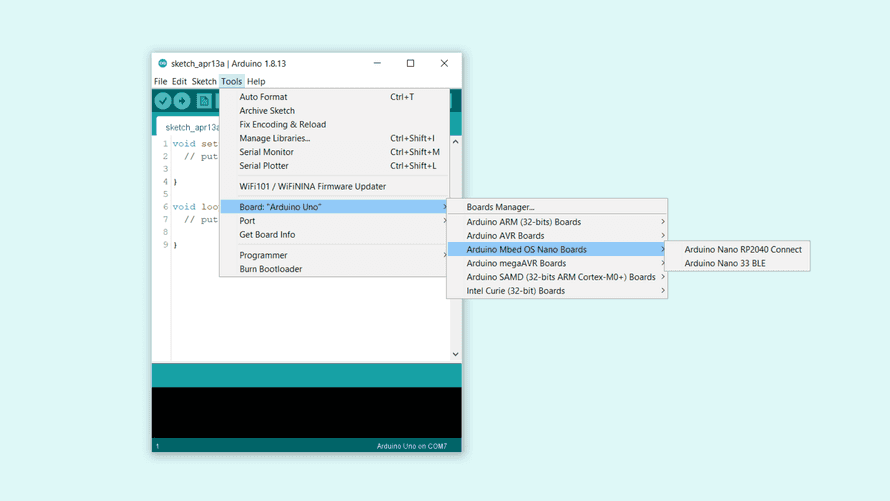
\includegraphics[width=0.7\textwidth]{Images/install_mbed_img04}
	\caption{Select the board}
	\label{fig:Check Board}
\end{figure}


\subsubsection{Select the Appropriate Port}

After selecting the Arduino nano 33 BLE sense board, next we need to check the connected port. For doing this, we need to set our arduino borad in Boot setup by clicking the white reset button on arduino as show in figure \ref{fig:Check-Reset}.

\begin{figure}[h]
	\centering
	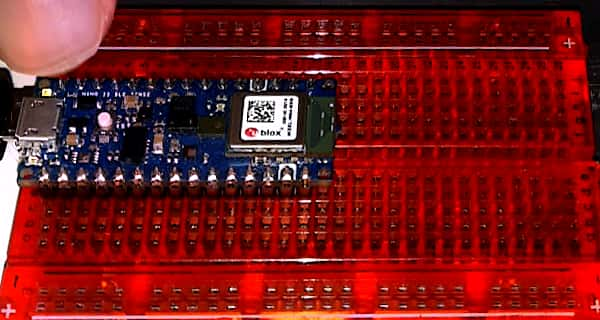
\includegraphics[width=0.7\textwidth]{Images/Click-Reset}
	\caption{Select the board}
	\label{fig:Check-Reset}
\end{figure}

By clicking the white reset button, the arduino borad will be in boot setup and make sure to check the orange LED glow as shown in the figure \ref{fig:LED-Glow}.

\begin{figure}[h]
	\centering
	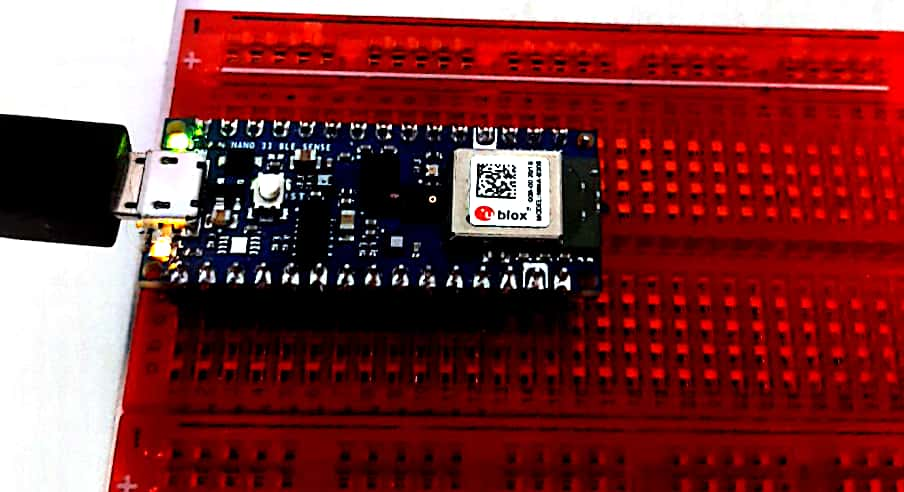
\includegraphics[width=0.7\textwidth]{Images/Orange LED}
	\caption{Orange LED Glow}
	\label{fig:LED-Glow}
\end{figure}

After successfully applying the above mention step, next we need to select the connected port before upload the program. For this, go to tool select arduino port and make sure to check it available port for uploading the program as shown in figure \ref{fig:Port-Selection}\cite{Arduino:2024g}

\begin{figure}[h]
	\centering
	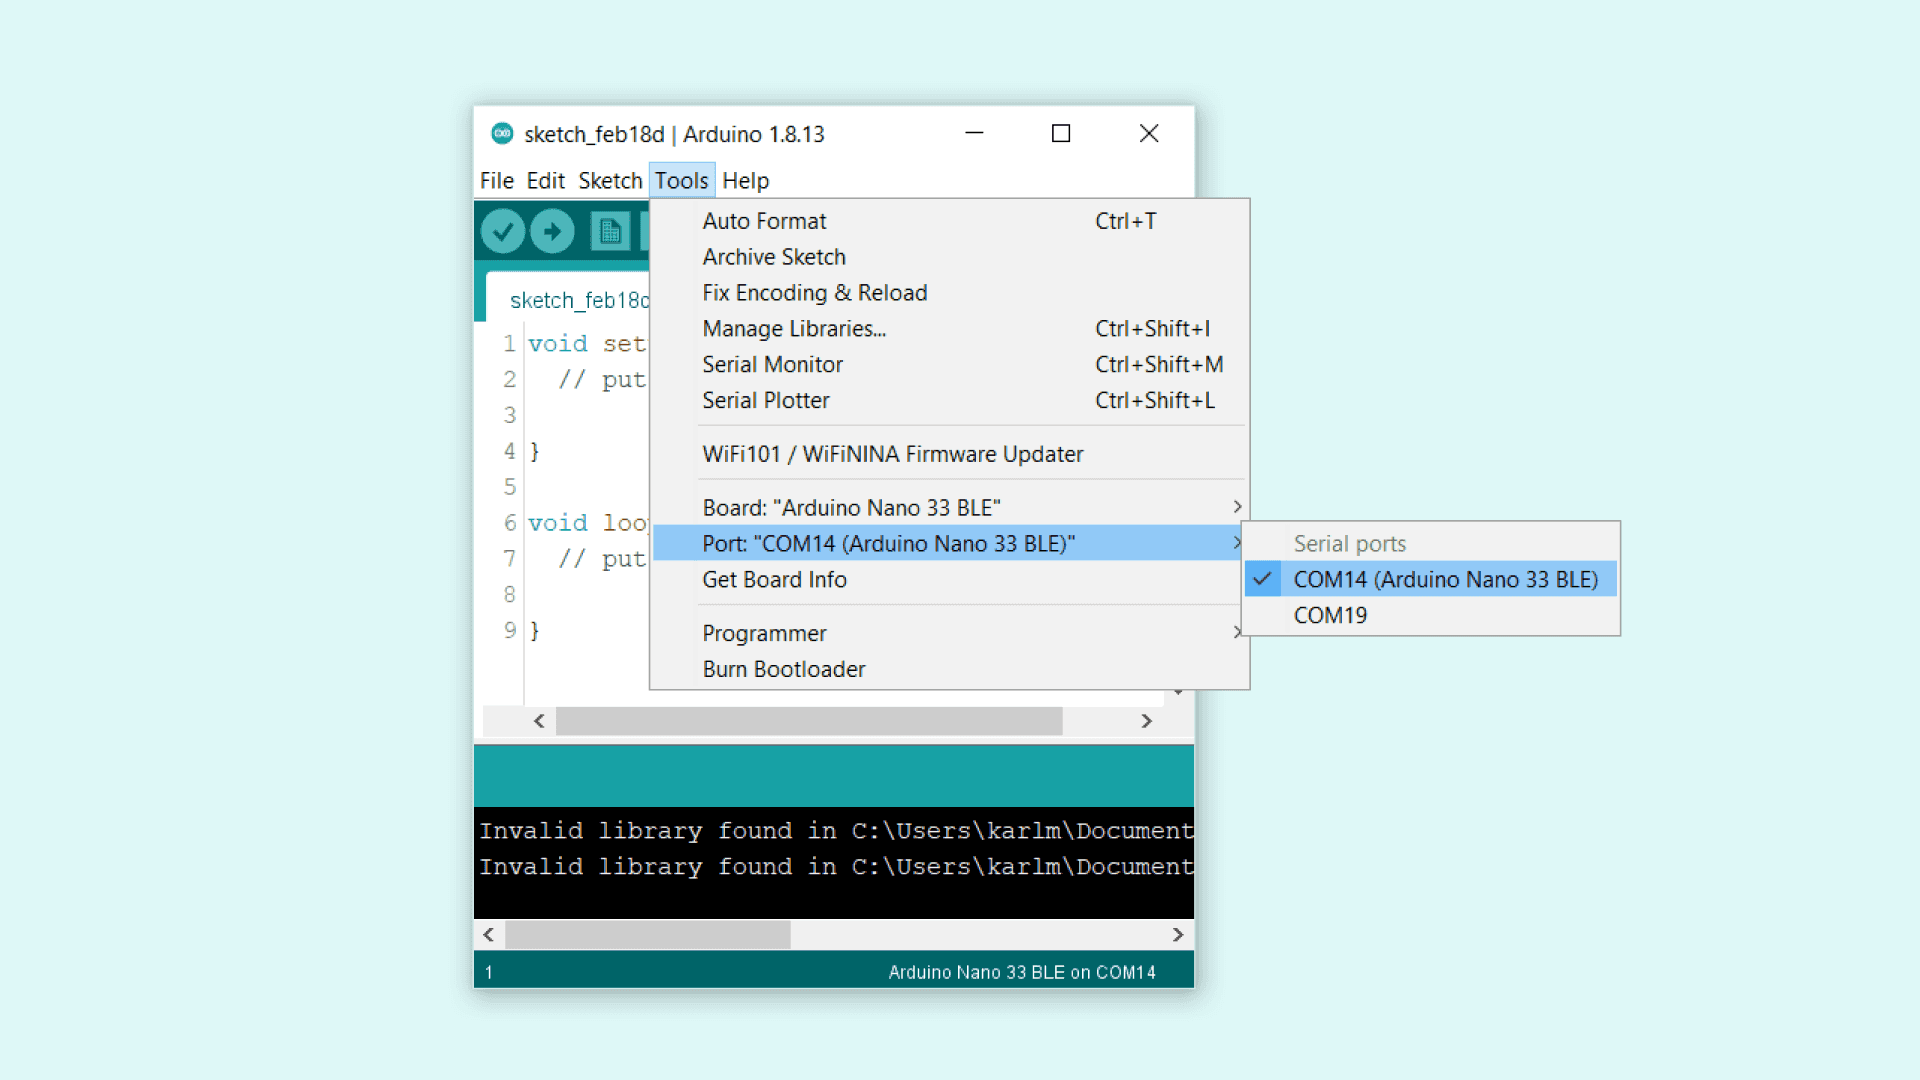
\includegraphics[width=0.7\textwidth]{Images/install_mbed_img05}
	\caption{Select Available Port for Uploading Arduino Sketch}
	\label{fig:Port-Selection}
\end{figure}

\subsubsection{Upload Code in Arduino Board}

After selecting the appropriate port, it's time to upload the Arduino program. There are five icons (verify, upload, new, open, save) below the file section, before uploading the program the best practice is to verify the program first, it show us if there are any error or warning in the program exist or not. By successfully verifying the program we can safely upload the program by click the upload button in the top below the file section as shown in figure. \ref{fig:Upload}.


\begin{figure}[h]
	\centering
	
	\caption{Upload the Program in Arduino board}
	\label{fig:Upload}
\end{figure}

After uploading, the code will compile and if there is any issue in our program it will pop up in the bottom black window as well.




